\documentclass[10pt]{article}

\usepackage[ngerman]{babel}
\usepackage[T1]{fontenc}
\usepackage[utf8]{inputenc}
\usepackage{booktabs}	%top + bot rule
\usepackage{array}	%multicolumn
\usepackage{tabularx}	% kp
\usepackage{dcolumn}	%Komma bündig
\usepackage{amsmath}
\usepackage[decimalsymbol=comma]{siunitx}
\usepackage{graphicx}


\title{Notizen}
%\author{Florian Webner}

\begin{document}
\maketitle


\begin{align*}
&\nu  \qquad  &\text{...kinematische Viskosität} \\
&\eta           &\text{...dynamische Viskosität}\\
&\eta _{Luft} &=	17,1 \cdot 10^{-6} \si{.Pa \cdot s} \\
&\eta _{Wasser} (20^\circ C) &= 10^{-3} \si{Pa \cdot s}
\end{align*}
\begin{align*}
\eta = \nu \varrho
\end{align*}
\begin{align*}
 \nu _{Luft} = 14,2 \cdot 10^{-6} \si{. \frac{m^2}{s}} \\
\nu _{Wasser} = 1 \cdot 10{-6}  \si{. \frac{m^2}{s}}
\end{align*}

\begin{align*}
R_e = \frac{UL}{\nu} \Rightarrow R_{e,Wasser} \approx 14 \cdot R_{e, Luft}\\
\text{(für gleiche Größe und gleiche Anströmgeschwindigkeit)}
\end{align*}

\begin{tabularx}{\linewidth}{ccp{3cm}c cp{3cm}}
\toprule
Körper 	&  Re & Aufhängung &	$C_w$ & $\text{V}_{schlepp}$ &Quelle\\	
 &							&			& &(20cm breit)   \\
\midrule
\medskip
Quader a)&	$1,7 \cdot 10^5$	& Mit Klavierdraht an einem T-Träger & 0,8-1,2	& 0,85 m/s &	Nakaguchi  (1978) \\
\medskip
Zylinder b) &$1 \cdot 10^5$ & schwebende Magnetaufhängung ohne Beeinflussung der Strömung & 0,85 & 0,5 m/s &Y. Kawamura: Wind Tunnel Experiment of Bluff
Body Aerodynamic (...)	\\
\medskip
Kugel c) & $1 \cdot 10^5$ & *wie Zylinder* & 0,5 & 0,5 m/s& *wie zylinder*  \\
\medskip
Zylinder d) & $9,4 \cdot 10^4$ & Hängt an 4 senkrechten Drähten (2 vorne , 2 hinten). Widerstandskraft aus Pendelauslenkung bestimmt & 0,2-0,6 & 0,47 m/s  & T. Morel: The effect of base slant on the flow pattern and drag of 3D bodies with blunt ends	\\
Ahmed-Body e) &$1,4 \cdot 10^6$ & auf 2 Stiften unter dem Objekt, in Bodennähe und Bodenabstand &0,2-0,4 & 7 m/s &T. Morel  *wie Zylinder d)*\\
\bottomrule


\end{tabularx}
\begin{figure}[h]

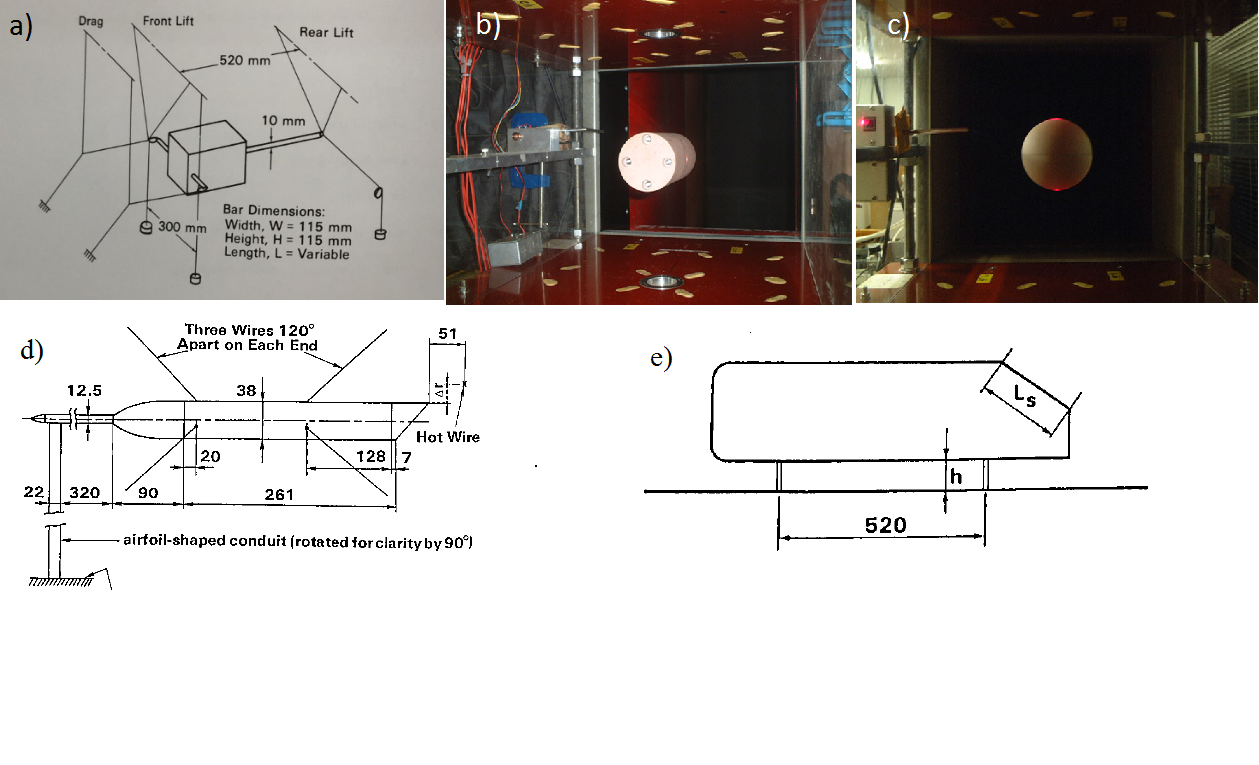
\includegraphics[width=\linewidth]{GrafikenKorper}
\end{figure}






	
\end{document}
